\documentclass{article}
\usepackage{enumerate}
\usepackage{amsmath}
\usepackage{amssymb}
\usepackage{graphicx}
\usepackage{subfigure}
\usepackage{geometry}
\usepackage{color}
\usepackage{bm}
\usepackage{indentfirst}
\usepackage{float}
\usepackage{booktabs}

\begin{document}

\vspace*{0.25cm}

\hrulefill

\thispagestyle{empty}

\begin{center}
\begin{large}
\sc{UM--SJTU Joint Institute \vspace{0.3em} \\ Physics Laboratory \\(VP241)}
\end{large}

\hrulefill

\vspace*{5cm}
\begin{Large}
\sc{{Laboratory Report}}
\end{Large}

\vspace{2em}

\begin{large}
\sc{{Exercise 1
\vspace{0.5em}

Basic Characteristics of Magnetic Materials
}}
\end{large}
\end{center}


\vfill

\begin{table}[h!]
\flushleft
\begin{tabular}{lll}
Name: Yihao Liu \hspace*{2em}&
ID: 515370910207\hspace*{2em}& Group: 7\\


\\

Date: 18 Nov 2016 

\end{tabular}
\end{table}

\hfill
\begin{tiny}
[rev. 1.0]
\end{tiny}

\newpage

\tableofcontents

\newpage

\section{Objectives}

The goal of this exercise is to study the shape of the magnetic hysteresis loop and the
magnetization curve, and understand how to use these characteristics to discuss properties
of ferromagnetic materials. In this exercise these properties will be studied quantitatively
using the concepts of the coercive field strength, the residual magnetic field and the
magnetic susceptibility. The magnetization curve and the magnetic hysteresis loop will
be visualized on the oscilloscope. Also, time permitting, the Curie temperature of a
ferromagnetic material will be found experimentally.



\section{Theoretical Background}

Magnetic materials are widely used in electric power industry, electronic devices, such
as computers, and in information storage technology. Their basic properties can be dis-
cussed by studying the magnetic hysteresis loop and measuring the Curie temperature.
The former provides information about how easy is to change properties of the magnetic
material, and the latter characterizes the phase transition between from/to the magnetically ordered phase.


\subsection{Magnetization}

Magnetic medium is defined as matter that can be magnetized, that is magnetic dipole
moments in the material can be arranged into some ordered pattern. The process of
magnetization can be described in terms of three quantities: the magnetic field B, the
magnetization M, and the auxiliary magnetic field H. In the simplest case, these three
quantities can be represented by their magnitudes and are related as follows

$$B=\mu_0(H+M)=(\chi_m+1)\mu_0H=\mu_r\mu_0H=\mu H$$

where $\mu_0 = 4\pi \cdot 10^{-7} H/m$ is the magnetic permeability of vacuum, $\chi_m$ is the magnetic
susceptibility of the material, the dimensionless quantity $\mu_r = \chi_m+1 = B=/\mu_0 $ is called the
relative magnetic permeability of the material, and $\mu = \mu_r\mu_0$ is the material's (absolute)
magnetic permeability. For a paramagnetic material, $\chi_m > 0$ and $\mu_r$ is slightly greater
than 1. On the other hand, for a diamagnetic material, $\chi_m < 0$ with the absolute value
between $10^{-4}$ and $10^{-5}$ and $\mu_r$ is slightly less than 1. For a ferromagnetic material,
$\chi_m \gg 1$, so that $\mu_r \gg 1$.

\begin{figure}[H]
	\centering
	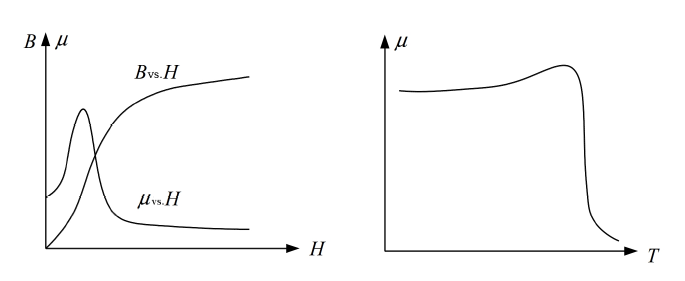
\includegraphics[scale=0.6]{fig1.png}
	\caption{(left) The magnetization curve B(H) for a ferromagnetic material and the
curve $\mu$(H). (right) A generic graph of the $\mu$(T) curve for a ferromagnetic material.}
\end{figure}

The magnitudes of the magnetic field and the auxiliary magnetic field are related
linearly in non-ferromagnetic isotropic materials, that is in such materials B = $\mu$H. How-
ever, for ferromagnetic materials the relationship is non-linear. In ferromagnetic materials
there is a spontaneous magnetization (magnetic dipole moments are spontaneously oriented parallel to each other) that increases with the decreasing temperature. Figure 1
(left) shows a typical magnetization curve B = B(H) with some features common to all
ferromagnetic materials. Namely, when H increases, B increases slowly at the beginning
and $\mu$ is small; then B and $\mu$ both rapidly increase as H increases; finally, B reaches a
saturation level and $\mu$ rapidly decreases after reaching a maximum value. Figure 1 indicates that the magnetic permeability $\mu$ is a function of both the auxiliary magnetic field
H (Figure 1, left) and the temperature T (Figure 1, right).

If the temperature is increased above a certain value, a ferromagnet will turn into a
paramagnet, that is a material with randomly oriented magnetic dipole moments. This
critical value of the temperature is called the Curie temperature, and on the graph $\mu$ vs.
T it is the temperature corresponding to the point where the slope of the tangent line is
maximum.

\subsection{Magnetic Hysteresis}
In addition to high magnetic permeability, ferromagnets have another important property, which is the magnetic hysteresis. When a ferromagnet is being magnetized, the
magnetic field B depends not only on the current value of the auxiliary magnetic field
H, but also on the previous state of the material, as shown in Figure 2. The curve OA,
where the magnetic field B grows as the auxiliary magnetic field H increases, describes
the process of magnetizing of an (initially demagnetized) ferromagnet. This curve is called the magnetization curve.

When the auxiliary magnetic field is increased to a certain value $H_S$, the magnetic eld
B hardly increases and reaches a saturation state. If then the auxiliary magnetic field is
being decreased, the magnetic field B is not decreasing along the original path, but rather choosing another path $AC''A'$. Furthermore, when H increases from the value $-H_S$, B
will reach A along the curve $A'CA$, and finally form a closed curve. When H = 0, we
have $|B|$ = $B_r$, where $B_r$ is called the remnant magnetic field (yielding the corresponding
remnant magnetization). In order to make B = 0, an auxiliary magnetic field has to
be applied in the reverse direction. When the auxiliary magnetic field reaches the value
$H = -H_C$, where $H_C$ is called the coercive field strength, the material is demagnetized
and the magnetic field B, and hence the magnetization, is zero.

\begin{figure}[H]
	\centering
	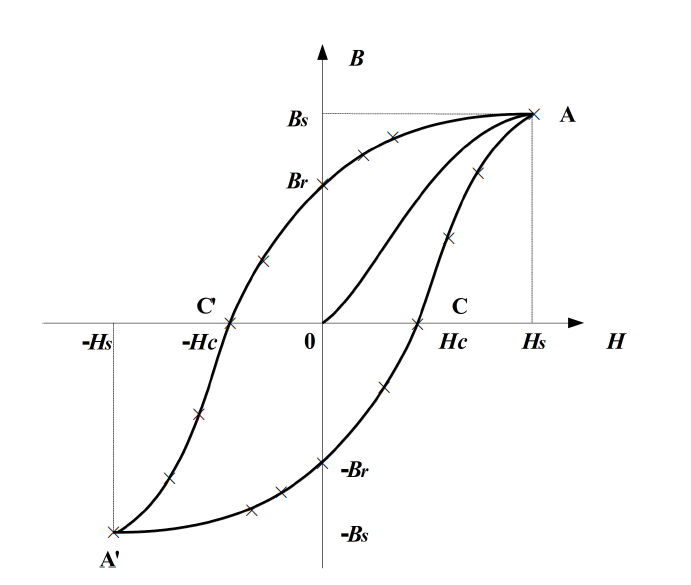
\includegraphics[scale=0.6]{fig2.png}
	\caption{The magnetization curve and the magnetic hysteresis loop of a ferromagnetic material. The crosses indicate the points to be recorded to describe the loop.}
\end{figure}


\subsection{Visualization on the Oscilloscope}

Figure 3 presents a diagram of a circuit that is used to visualize the magnetization
curve and the magnetic hysteresis loop on the oscilloscope. In this exercise they are
studied for a ferromagnet sample that has an average magnetic path of L and the number
of the turns in the coil is $N_1$. If the electric current through the coil is $i_1$, then according
to Ampere's law

$$HL=N_1i_1$$

In this case the input voltage for the deflection plate of the x axis channel of the oscilloscope is

$$U_{R_1}=R_1i_1=\frac{R_1L}{N_1}H$$

where $R_1$, $L$, and $N_1$ are constant. Hence, the input voltage for the x axis channel is
proportional to the auxiliary magnetic field H.

If the cross-sectional area of the sample is S, then according to the law of electromagnetic induction, the induced electromotive force in a secondary coil with the number of turns $N_2$, is

\begin{equation}
\varepsilon_2=-N_2S\frac{dB}{dt}
\end{equation}

Assuming that the number of turns $N_2$ in the secondary coil is small, the electromotive
force due to self-induction can be ignored. Moreover, if the values of the resistance $R_2$ and the capacitance C are chosen so that $R2 \gg 1/\omega C$, then

\begin{equation}
\varepsilon_2=R_2i_2
\end{equation}

Substituting $i_2=dq/dt=CdU_C/dt$ into Eq. (2) and combining with Eq. (1) one obtains

\begin{equation}
U_C=-\frac{N_2SB}{R_2C}
\end{equation}

which shows that the input voltage $U_C$ for the y axis channel is proportional to the
magnetic field B.

\begin{figure}[H]
	\centering
	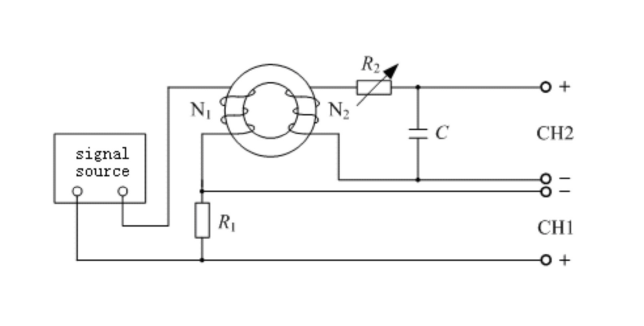
\includegraphics[scale=0.6]{fig3.png}
	\caption{The electric circuit for visualization of the magnetization curve and the magnetic hysteresis loop on the oscilloscope. $R_1 = 10\Omega$ and $R_2$ is a variable resistor with maximum resistance of $2.2k\Omega$.}
\end{figure}

\section{Measurement Setup and Procedure}

\subsection{Apparatus}

The apparatus for this exercise consists of the following main elements: a signal generator, an oscilloscope, a digital multimeter, a platinum resistance thermometer, a glass vacuum-tube heating pipe, a voltage/current source, a wiring block, a capacitor, two 200$\Omega$ resistors, a 10$\Omega$  resistor, a 2.2k$\Omega$ variable resistor, and a 1 k$\Omega$ resistor (the actual values of the resistance should be measured during the session). Ferromagnetic samples will be provided by the instructor.

The parameters of other elements are: $L = 3.61 \times 10^{-2} m$, $S = 1.25 \times 10^{-5} m^2$ and
$N_1 = N_2 = 100$. The capacity is indicated on the capacitor.

\subsection{Measurement Procedure}

\subsubsection{Magnetic Hysteresis Loop Measurement}
\begin{enumerate}
	\item Assemble the circuit according to Figure 3 with the signal source disconnected.
	\item Turn on the signal source and adjust the frequency to 1 kHz or above. Keep in
mind that you must not short the signal source, or set the frequency below 1 kHz
(otherwise the equipment will be damaged).
	\item Connect the signal source to the circuit and observe the $U_{R_1}$ vs. $U_C$ loop under different conditions:
	\item
	\begin{enumerate}[(1)]
		\item with different signal frequencies (1 ~ 2 kHz) and amplitudes (1 ~ 5 V),
		\item with different values of the resistance $R_2$.
	\end{enumerate}
	\item Obtain the saturated hysteresis loop for a certain frequency (1 ~ 2 kHz) and
suitable value of the resistance $R_2$ (about 1 k$\Omega$); shift the picture of the loop to the center of the oscilloscope screen, adjust its size and show the visualization to the instructor.
	\item Trace the whole loop with no less than 16 points (see Figure 2 for the location of the points).
	\item Turn off the signal source, disconnect the circuit and measure the resistances.
	\item After class, plot the magnetic hysteresis loop (H-B loop), and find $\pm B_r$, $\pm H_c$, $\pm B_s$, $\pm H_s$.
\end{enumerate}

\section{Results}

\subsection{Magnetic Hysteresis Loop Measurement}

\begin{table}[!h]
\begin{center}
\begin{tabular}{|c|c|}
\hline
$N_1$	&	100\\
\hline
$N_2$	&	100\\
\hline
$R_1$	&	10.17 $\pm$ 0.01 [$\Omega$]\\
\hline
$R_2$	&	992.9 $\pm$ 0.1 [$\Omega$]\\
\hline
$L$		&	$3.61\times10^{-2}\pm10^{-4}$ [m]\\
\hline
$S$		&	$1.25\times10^{-5}\pm1-^{-7}$ [$\rm m^2$]\\
\hline
$C$		&	4.334 $\pm$ 0.001 [$\mu$F]\\
\hline
\end{tabular}
\caption{Parameters of circuit components (cf. Figure 3).}
\label{tab-1}
\end{center}
\end{table}

\begin{table}[!h]
\begin{center}
\begin{tabular}{|c|c|c|c|c|c|c|}
\hline
$U_{R_1}(\pm0.5\ [mV])$	&	-213.0	&	-150.0	&	-100.0	&   -50.0	&	 0.0	&	 50.0	\\
\hline
$U_{C}(\pm0.5\ [mV])$	& 	 139.0 	&	 131.5 	&	 123.0	&	 110.0	&	 90.0	&	 53.0	\\
\hline
$U_{R_1}(\pm0.5\ [mV])$	&	 72.5	&	 100.0	&	 150.0	&	 212.0	&	 150.0	&	 100.0	\\
\hline
$U_{C}(\pm0.5\ [mV])$	&	 0.0	&	-80.5	&	-116.5	&   -134.0	&	-127.5	&	-118.0	\\
\hline
$U_{R_1}(\pm0.5\ [mV])$	&	 50.0	&	 0.0	&	-44.5	&	-101.0	&	-91.0	&	-150.0	\\
\hline
$U_{C}(\pm0.5\ [mV])$	&	-104.5	&	-82.5	&	-43.5	&	 0.0	&	 84.5	&	 121.0	\\
\hline
\end{tabular}
\caption{Oscilloscope measured values of $U_{R_1}$ and $U_C$ in the circuit illustrated in Figure 3.}
\label{tab-2}
\end{center}
\end{table}

\newpage

The data of H and B was calculated and shown in Table 3.

\begin{table}[!h]
\begin{center}
\begin{tabular}{|c|c|c|}
\hline
No & H [T] & B [$1\times10^3$ T] \\
\hline
1	&	$-58.02\pm	0.22$	&	$-478.52\pm	4.20$	\\
\hline
2	&	$-40.86\pm	0.18$	&	$-452.70\pm	4.01$	\\
\hline
3	&	$-27.24\pm	0.16$	&	$-423.44\pm	3.80$	\\
\hline
4	&	$-13.62\pm	0.14$	&	$-378.68\pm	3.49$	\\
\hline
5	&	$0.00\pm	0.14$	&	$-309.83\pm	3.02$	\\
\hline
6	&	$13.62\pm	0.14$	&	$-182.46\pm	2.26$	\\
\hline
7	&	$19.75\pm	0.15$	&	$-0.00\pm	1.72$	\\
\hline
8	&	$27.24\pm	0.16$	&	$277.13\pm	2.81$	\\
\hline
9	&	$40.86\pm	0.18$	&	$401.06\pm	3.64$	\\
\hline
10	&	$57.74\pm	0.22$	&	$461.31\pm	4.07$	\\
\hline
11	&	$40.86\pm	0.18$	&	$438.93\pm	3.91$	\\
\hline
12	&	$27.24\pm	0.16$	&	$406.22\pm	3.68$	\\
\hline
13	&	$13.62\pm	0.14$	&	$359.75\pm	3.35$	\\
\hline
14	&	$0.00\pm	0.14$	&	$284.01\pm	2.85$	\\
\hline
15	&	$-12.12\pm	0.14$	&	$149.75\pm	2.10$	\\
\hline
16	&	$-16.62\pm	0.14$	&	$-0.00\pm	1.72$	\\
\hline
17	&	$-24.79\pm	0.15$	&	$-290.90\pm	2.90$	\\
\hline
18	&	$-40.86\pm	0.18$	&	$-416.55\pm	3.75$	\\
\hline
\end{tabular}
\caption{The data of H and B.}
\label{tab-3}
\end{center}
\end{table}


The figure was plotted in Figure 4.

\begin{figure}[H]
	\centering
	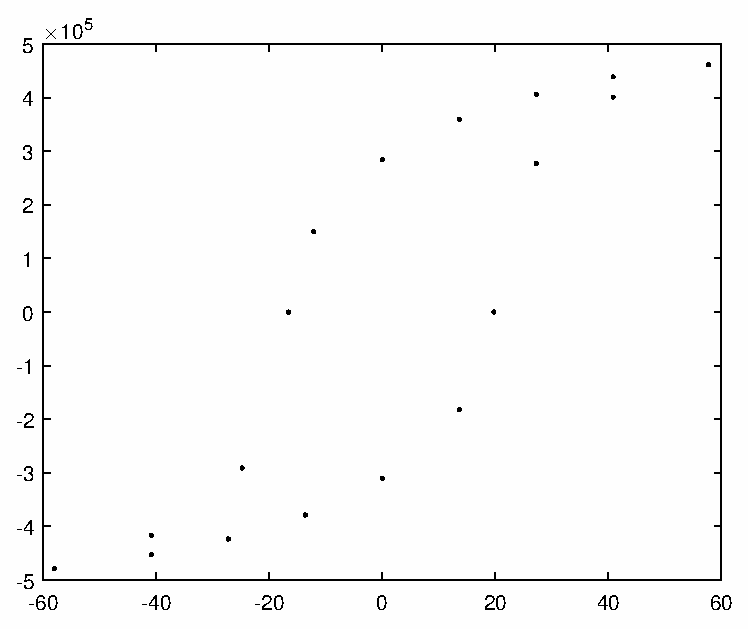
\includegraphics[scale=0.6]{fig.eps}
	\caption{H vs. B graph.}
\end{figure}

\section{Measurement uncertainty analysis}

\subsection{Relation Between Sensitivity $ K_H $ and Working Voltage $ U_S $}

$H$ can be calculated by the equation $H=\frac{N_1U_{R_1}}{R_1L}$. Therefore its uncertainty $u_{H}$ is found by applying the uncertainty propagation formula

\begin{align*}
u_{H}&=\sqrt{\left(\frac{\partial H}{\partial U_{R_1}}\right)^2u_{U_{R_1}}^2+\left(\frac{\partial H}{\partial R_1}\right)^2u_{R_1}^2+\left(\frac{\partial H}{\partial  L}\right)^2u_L^2}\\
&=N_1\sqrt{\left(\frac{1}{R_1L}\right)^2u_{U_{R_1}}^2+\left(\frac{U_{R_1}}{R_1^2L}\right)^2u_{R_1}^2+\left(\frac{U_{R_1}}{R_1L^2}\right)^2u_{L}^2}\\
\end{align*}

$B$ can be calculated by the equation $B=-\frac{R_2CU_C}{N_2S}$. Therefore its uncertainty $u_{B}$ is found by applying the uncertainty propagation formula

\begin{align*}
u_{B}&=\sqrt{\left(\frac{\partial B}{\partial R_2}\right)^2u_{R_2}^2+\left(\frac{\partial B}{\partial C}\right)^2u_{C}^2+\left(\frac{\partial B}{\partial U_C}\right)^2u_{U_C}^2+\left(\frac{\partial B}{\partial S}\right)^2u_{S}^2}\\
&=\frac{1}{N_2}\sqrt{\left(\frac{CU_C}{S}\right)^2u_{R_2}^2+\left(\frac{R_2U_C}{S}\right)^2u_{C}^2+\left(\frac{R_2C}{S}\right)^2u_{U_C}^2+\left(\frac{R_2CU_C}{S^2}\right)^2u_{S}^2}\\
\end{align*}


\section{Conclusion}

In this lab, I studied the shape of the magnetic hysteresis loop and the
magnetization curve, and understand how to use these characteristics to discuss properties of ferromagnetic materials.

According to the two equations

$$H=\frac{N_1U_{R_1}}{R_1L}$$

$$B=-\frac{R_2CU_C}{N_2S}$$

We can get the linear relationship between the value we measured on the oscilloscope and the real strength of magnetic fields.

\section{Reference}

\begin{enumerate}[(a)]
	\item
	Qin Tian, Zeng Ming, Mateusz Krzyzosiak, VP241 Exercise 1, Basic Characteristics of Magnetic Materials, based on materials provided by the Department of Physics, Shanghai Jiaotong University.
\end{enumerate}

\section{Data sheet}

The Data sheet is attached at the end of the report.

\end{document}
